\newpage
\section{Auswertung}
\label{sec:Auswertung}
\subsection{Verstärkung eines gestörten Signales}
%Der erste Teil der verwendeten Maschine, der Funktionsgenerator, hat einen Ausgang für Spannung, 
%die in Amplitude, Spannungsform und Frequenz angepasst werden kann, und einen Ausgang, 
%der parallel zum ersten Ausgang die gleiche Spannungsform und Frequenz bei konstanter Amplitude liefert.
Die Amplitude bei Sinus-förmiger Wechselspannung ist an beiden Ausgängen \SI{0}{\volt}.
%Weiter wird das Messsignal über einen Verstärker verstärkt und mithilfe eines Bandpasses gefiltert, während das Referenzsignal in einen Phasenwandler geleitet wird.
%Beide Signale werden anschließend in dem Lock-In-Detektor gemischt und
\begin{table}
	\centering
	\begin{tabular}{c S[table-format=1.2]S[table-format=1.2]}
	\toprule
	{Phase}&\multicolumn{2}{c}{Ausgangsspannung in V}\\
	&{ohne Störung}&{mit Störung}\\
	\midrule
		0°		&-6.00	& 6.00\\
		45°		&-4.00	& 4.00\\
		90°		& 0.20	&-0.50\\
		120°	& 2.62	&-3.00\\
		135°	& 4.25	&-4.50\\
		180°	& 5.81	&-6.00\\
		225°	& 3.95	&-3.50\\
		270°	& 0.20	& 0.50\\
		315°	&-4.17	& 4.50\\
		360°	&-5.83	& 5.50\\
	\bottomrule
	\end{tabular}
	\caption{Ausgangsspannung des gegebenen Signals.}
	\label{tab:spannung}
\end{table}
Die Spannungen, die der den Tiefpass, das letzte Bauelement des Lock-In-Verstärkers, verlassen, sind in Tabelle \ref{tab:spannung} aufgetragen. 
Die angegebene Phase ist die eingestellte Phase des Phasenschiebers.
Diese Spannungen werden in Diagramm \ref{diag:spannung} gegen die eingestellte Phase aufgetragen; 
es zeigt sich, dass die Beziehung \eqref{cosinus_ausgangsspannung} durch die Datenpunkte verifiziert wird, es aber zu einem festen Phasenversatz $\alpha$ von $\alpha=\pi$ kommt.
Dieser Phasenversatz $\alpha$ ist bei dem Verfahren mit gestörtem Signal nicht existent.
Das Diagramm \ref{diag:stoerung} zeigt die Beziehung \eqref{cosinus_ausgangsspannung} deutlich.
\begin{figure}[hp]
	\centering
	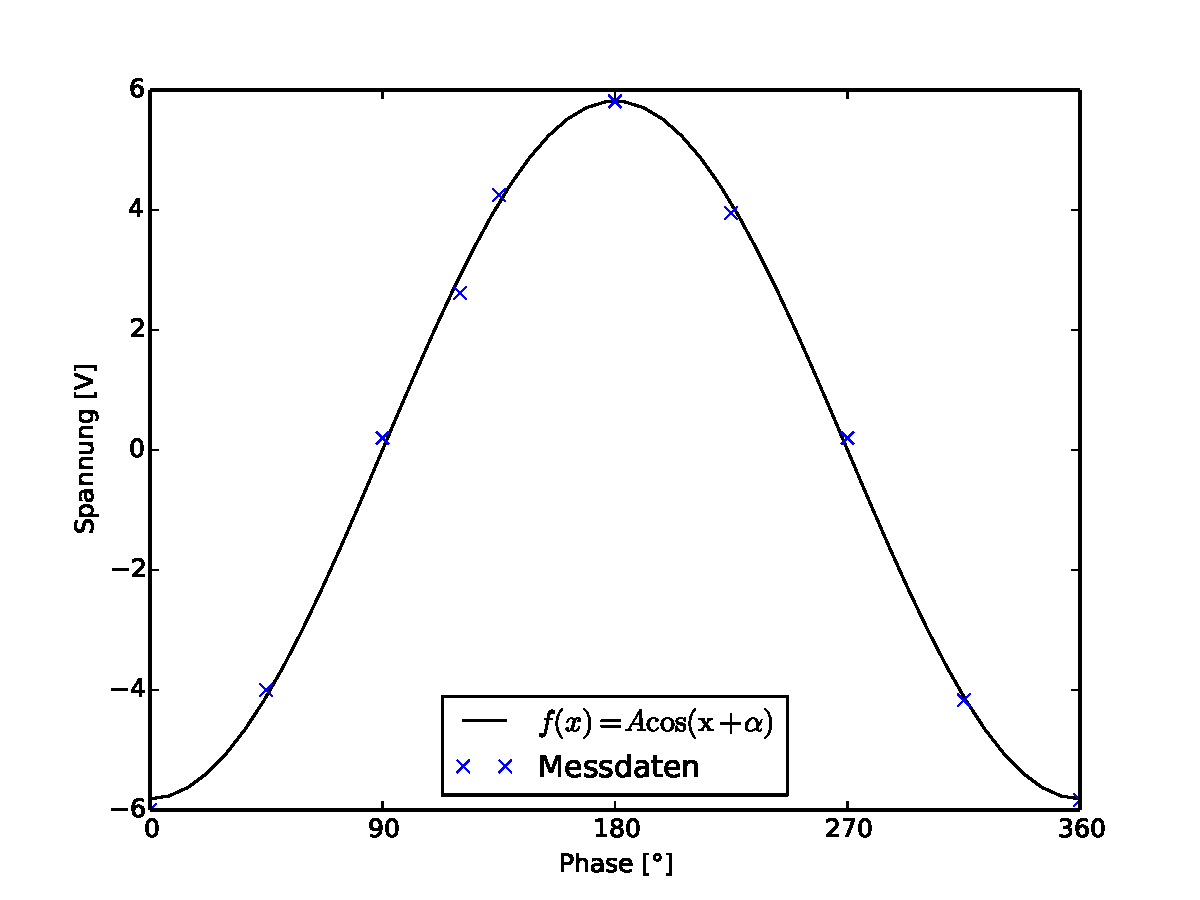
\includegraphics[width=0.8\textwidth]{Bilder/AusgangSpannung.pdf}
	\caption{Ausgangsspannung des Lock-In-Verstärkers bei Sinus-förmigen Eingang mit $U = \SI{0}{\volt}$ und $f = \SI{300}{\hertz}$.}
	\label{diag:spannung}
\end{figure}

\begin{figure}[hp]
	\centering
	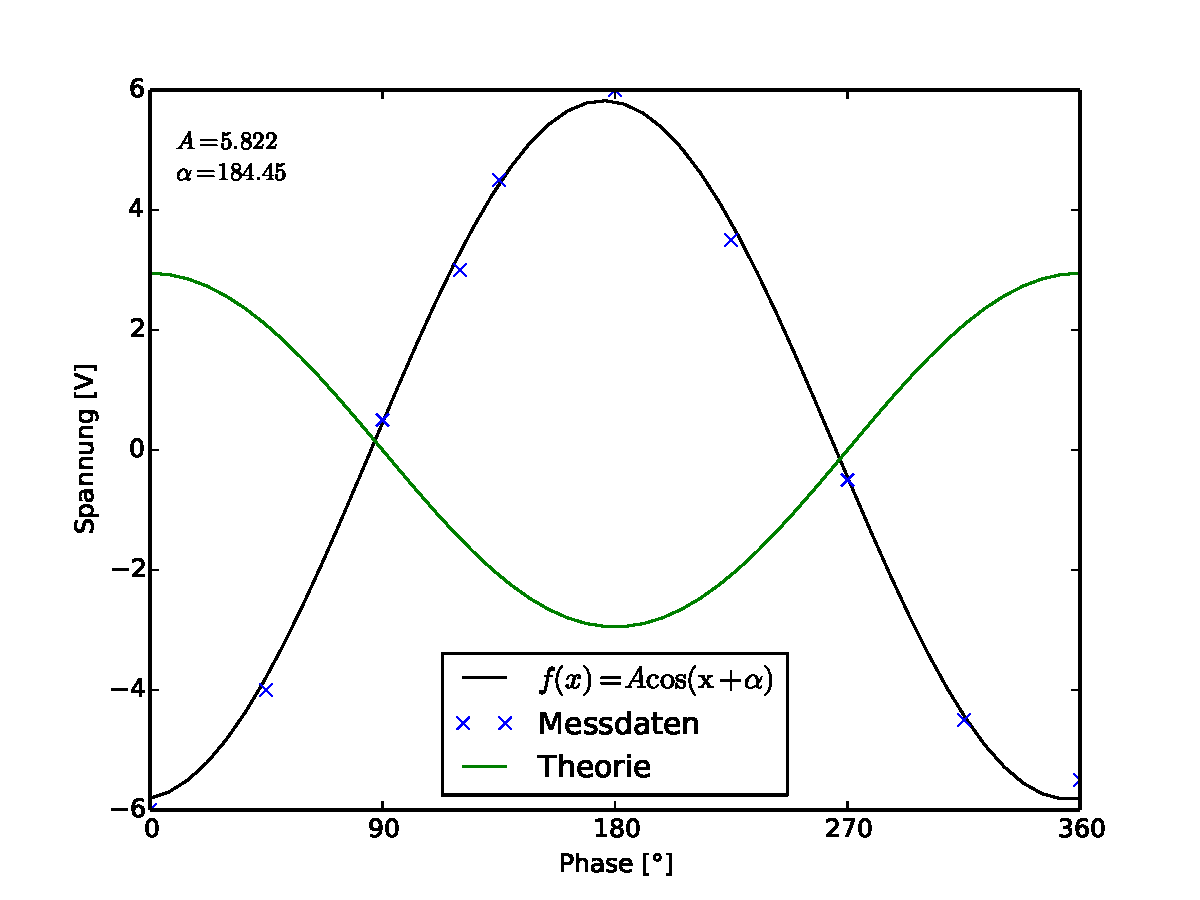
\includegraphics[width=0.8\textwidth]{Bilder/AusgangStoerung.pdf}
	\caption{Ausgangsspannung des Lock-In-Verstärkers bei gestörtem Signal.}
	\label{diag:stoerung}
\end{figure}

\begin{figure}[htbp]
	\begin{subfigure}{0.45\textwidth}
		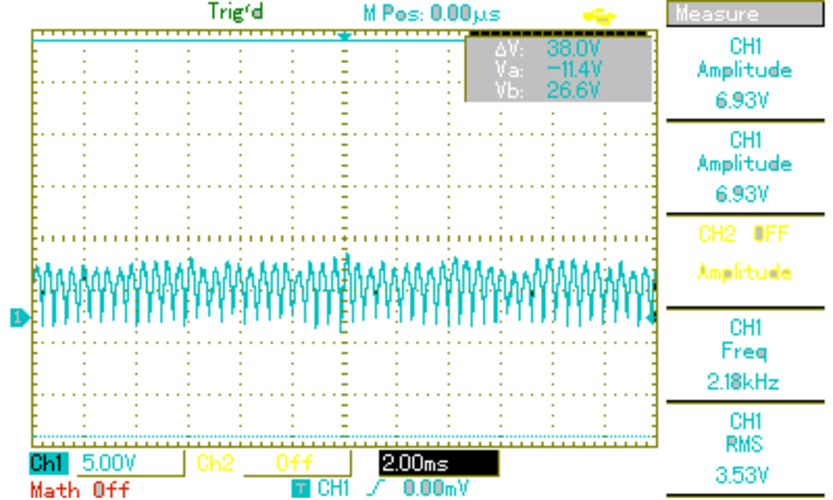
\includegraphics[width=\textwidth]{Bilder/MAP002.pdf}
	\end{subfigure}
	\begin{subfigure}{0.45\textwidth}
		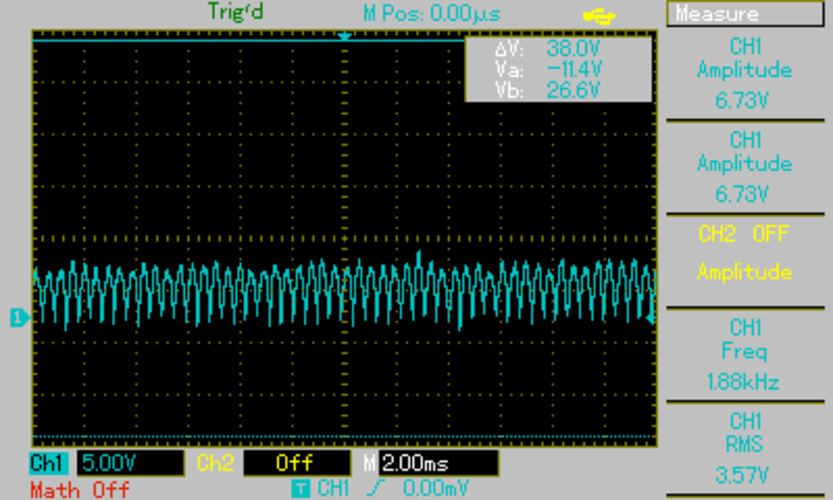
\includegraphics[width=\textwidth]{Bilder/MAP003.pdf}
	\end{subfigure}
	\caption{Das Signal mit Störungen zu zwei verschiedenen Zeiten.}
	\label{fig:stoerung}
\end{figure}
\subsection{Verstärkung des LED-Signales}
\begin{table}
	\centering
	\begin{tabular}{c S[table-format=1.2] l c}
	\toprule
	{Abstand a $/\si{\meter}$}&{Ausgangsspannung}&\multicolumn{2}{c}{Gesamt-Verstärkung}\\
	{}&{$\/\si{\volt}$}&{absolut}&{relativ}\\
	\midrule
		0.02&	-5 		& $400\cdot5$ 	 & 1\\
		0.05&	-1 		& $400\cdot5$ 	 & 1\\
		0.08&	-0.5 	& $400\cdot5$ 	 & 1\\
		0.11&	-2 		& $400\cdot50$ 	 & 10\\
		0.14&	-1 		& $400\cdot50$	 & 10\\
		0.17&	-0.9 	& $400\cdot50$	 & 10\\
		0.20&	-6.0	& $400\cdot500$	 & 100\\
		0.23&	-4.5 	& $400\cdot500$	 & 100\\
		0.26&	-3.5 	& $400\cdot500$	 & 100\\
		0.29&	-2.5 	& $400\cdot500$	 & 100\\
		0.39&	-1.0 	& $400\cdot500$	 & 100\\
		0.49&	-0.7 	& $400\cdot500$	 & 100\\
		0.59&	-0.5 	& $400\cdot500$	 & 100\\
		0.69&	-0.3 	& $400\cdot500$	 & 100\\
		0.79&	-0.25 	& $400\cdot500$	 & 100\\
		0.99&	-0.12 	& $400\cdot500$	 & 100\\
		1.19&	-0.1 	& $400\cdot500$	 & 100\\
	\bottomrule
	\end{tabular}
	\caption{Ausgangsspannung bei der Messung des LED-Lichtes.}
	\label{tab:led}
\end{table}
Bei einem messbaren Signal geht die Ausgangsspannung auf Null zurück, wenn die LED abgedeckt wird.
Bei einem Abstand von $\SI{1.20}{\meter}$ ist keine messbare Ausgangsspannung messbar, 
die angegebene Ausgangsspannung zeigt beim Abdecken der LED keine wesentliche Änderung.

\begin{figure}[hp]
	\centering
	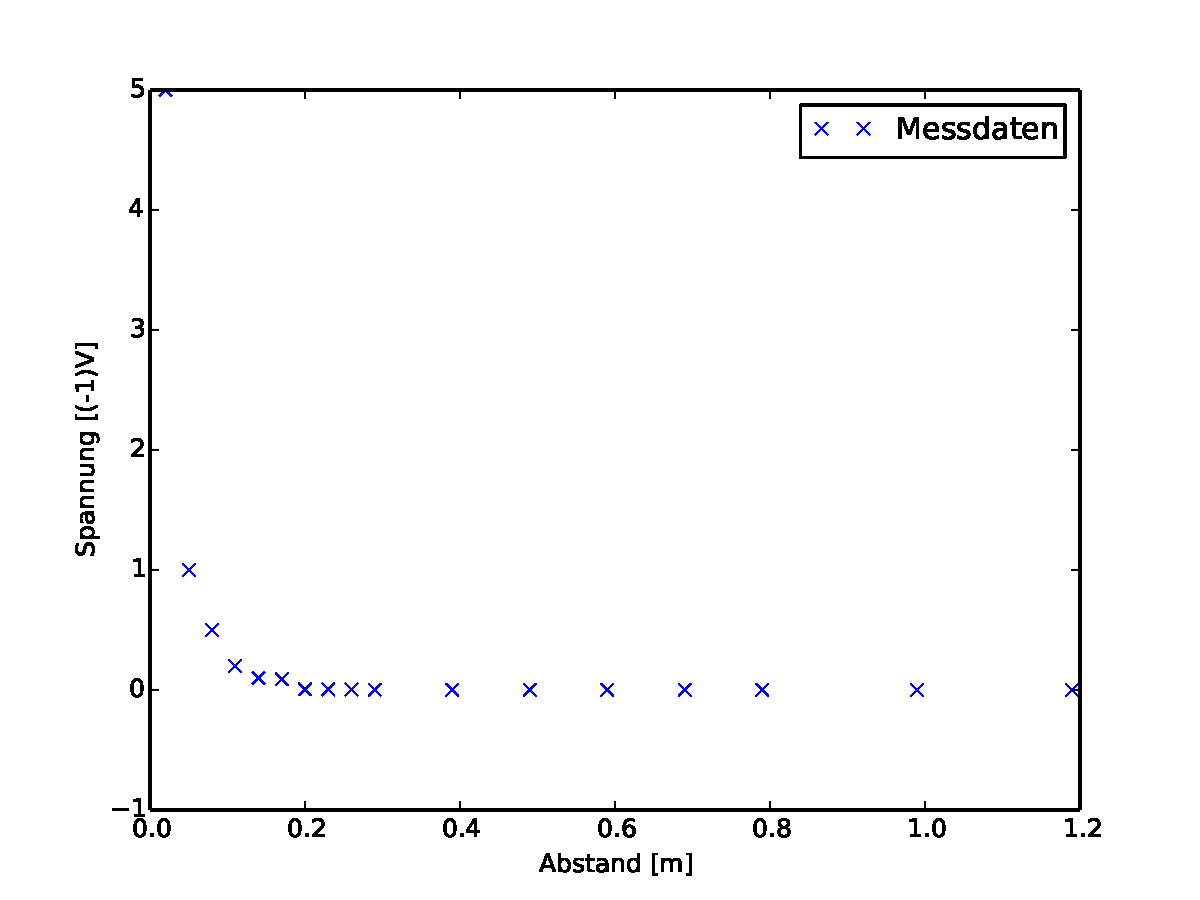
\includegraphics[width=0.8\textwidth]{Bilder/LED.pdf}
	\caption{Ausgangsspannung des Lock-In-Verstärkers bei gestörtem Signal.}
	\label{diag:LED}
\end{figure}